\documentclass[12pt]{article}

\usepackage[a4paper, margin=2.5cm]{geometry}
\usepackage{graphicx}
\usepackage{fontenc}
\usepackage{inputenc}
\usepackage{setspace}
\usepackage{hyperref}
\usepackage{setspace}
\usepackage{booktabs}
\usepackage{caption}
\usepackage{subcaption}
\usepackage{amsmath}
\usepackage{hyperref}

\begin{document}

\begin{titlepage}
    \centering

    % University logo
    
\includegraphics[width=0.45\textwidth]{images/ozu_logo.png}\\[3cm]

    % Course
    {\large \textbf{EE 350 -- Electronics II}}\\[1cm]

    % Semester
    {\large \textbf{Spring 2025/26}}\\[1cm]

    % Lab number
    {\large \textbf{LAB 3}}\\[1cm]

    % Lab title
    {\large \textbf{CMOS INVERTER AND RING OSCILLATOR}}\\[5cm]

    % Submission info
    \begin{center}
        {\normalsize \textbf{Submitted by:} Ömer Faruk AVCI}\\[0.4cm]
        {\normalsize \textbf{Student ID:} S034113}\\[0.4cm]
        {\normalsize \textbf{Date of Submission:} \today} 
    \end{center}

\end{titlepage}

% Introduction
\section*{Introduction}
In this laboratory session, we implemented and analyzed two fundamental CMOS circuits. In the first part, a physical CMOS inverter was constructed using discrete ZVP3306 PMOS and 2N7000 NMOS transistors to observe its switching behavior. The effect of different load capacitances ($1\ \mu\text{F}$, $2.2\ \mu\text{F}$, and $220\ \mu\text{F}$) on the output voltage transition and full-swing capabilities was evaluated. In the second part, a multi-stage ring oscillator was constructed using the SN7404 hex inverter IC.

\newpage
% Experiments 
\section*{Experiments}
\subsection*{Part 1: CMOS Inverter with Discrete Transistors}

A CMOS inverter was constructed on the breadboard by shorting the gates of the PMOS (ZVP3306) and NMOS (2N7000) transistors to form the input, and shorting their drains to form the output. The PMOS source was connected to $V_{DD} = 10\text{V}$ and the NMOS source to ground. A $10\text{V}$ peak-to-peak, $1\text{ kHz}$ square wave was applied to the input with a $5\text{V}$ DC offset to ensure the input signal strictly alternated between $0\text{V}$ and $10\text{V}$.

\subsubsection*{Task 1.1: $1\ \mu\text{F}$ Capacitor Load}
First, a $1\ \mu\text{F}$ capacitor was connected to the output terminal. The input and output voltage waveforms were observed on the oscilloscope as shown in Figure 1.

\begin{figure}[h]
        \centering
        % Replace with your image filename
        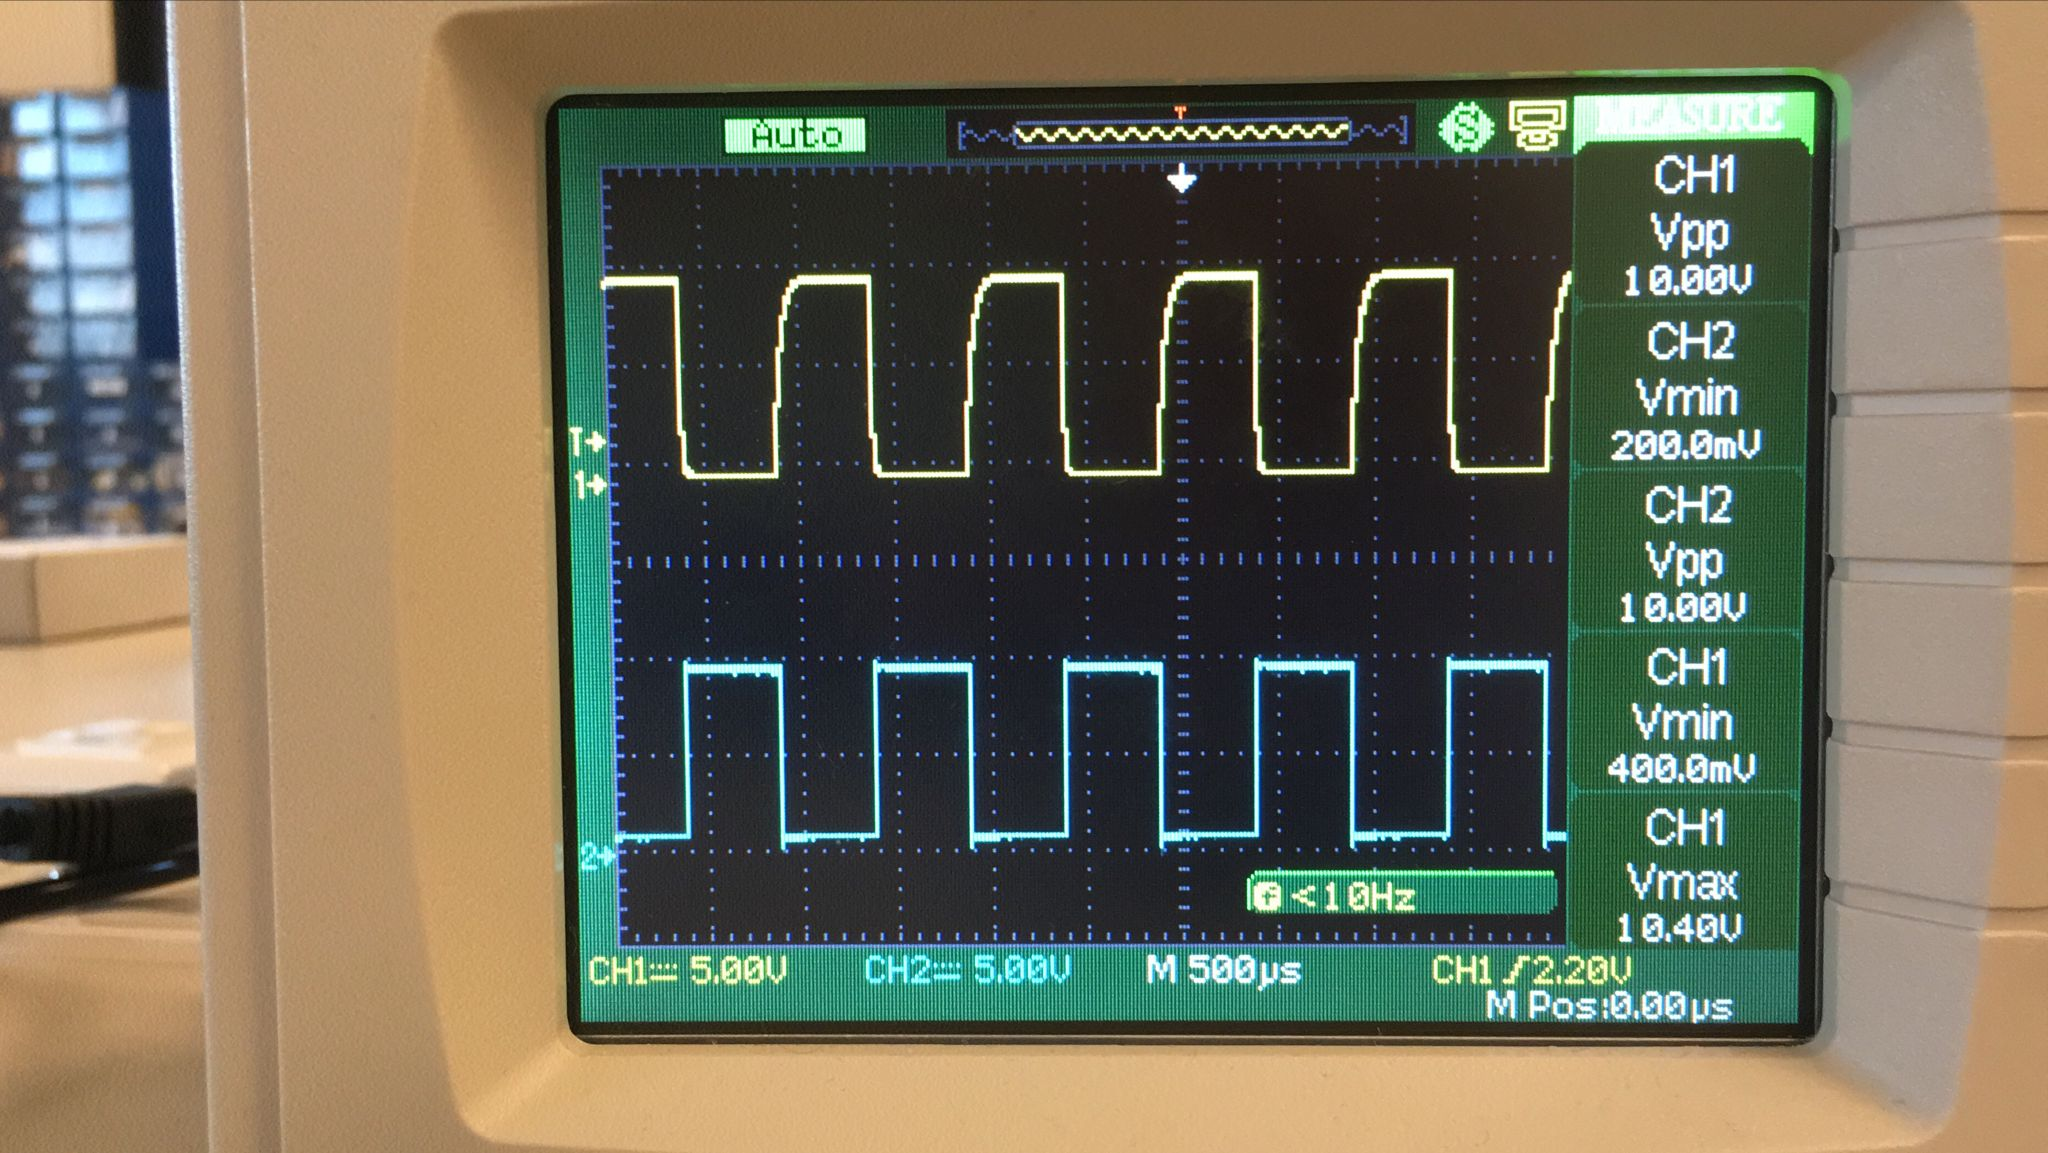
\includegraphics[width=0.75\linewidth]{images/task1_1uf.png} 
    \caption{Inverter Waveform with $1\ \mu\text{F}$ Capacitive Load}
\end{figure}

As seen in the waveform, when the input transitions to HIGH ($10\text{V}$), the NMOS conducts, pulling the output LOW. When the input goes LOW ($0\text{V}$), the PMOS conducts, charging the capacitor to $10\text{V}$. With $1\ \mu\text{F}$, the output manages to reach the full rail voltages ($0\text{V}$ and $10\text{V}$) comfortably before the next transition.
\newpage
\subsubsection*{Task 1.2: $2.2\ \mu\text{F}$ Capacitor Load}
The load was then increased to a $2.2\ \mu\text{F}$ capacitor. The resulting waveform is presented in Figure 2.

\begin{figure}[h]
        \centering
        % Replace with your image filename
        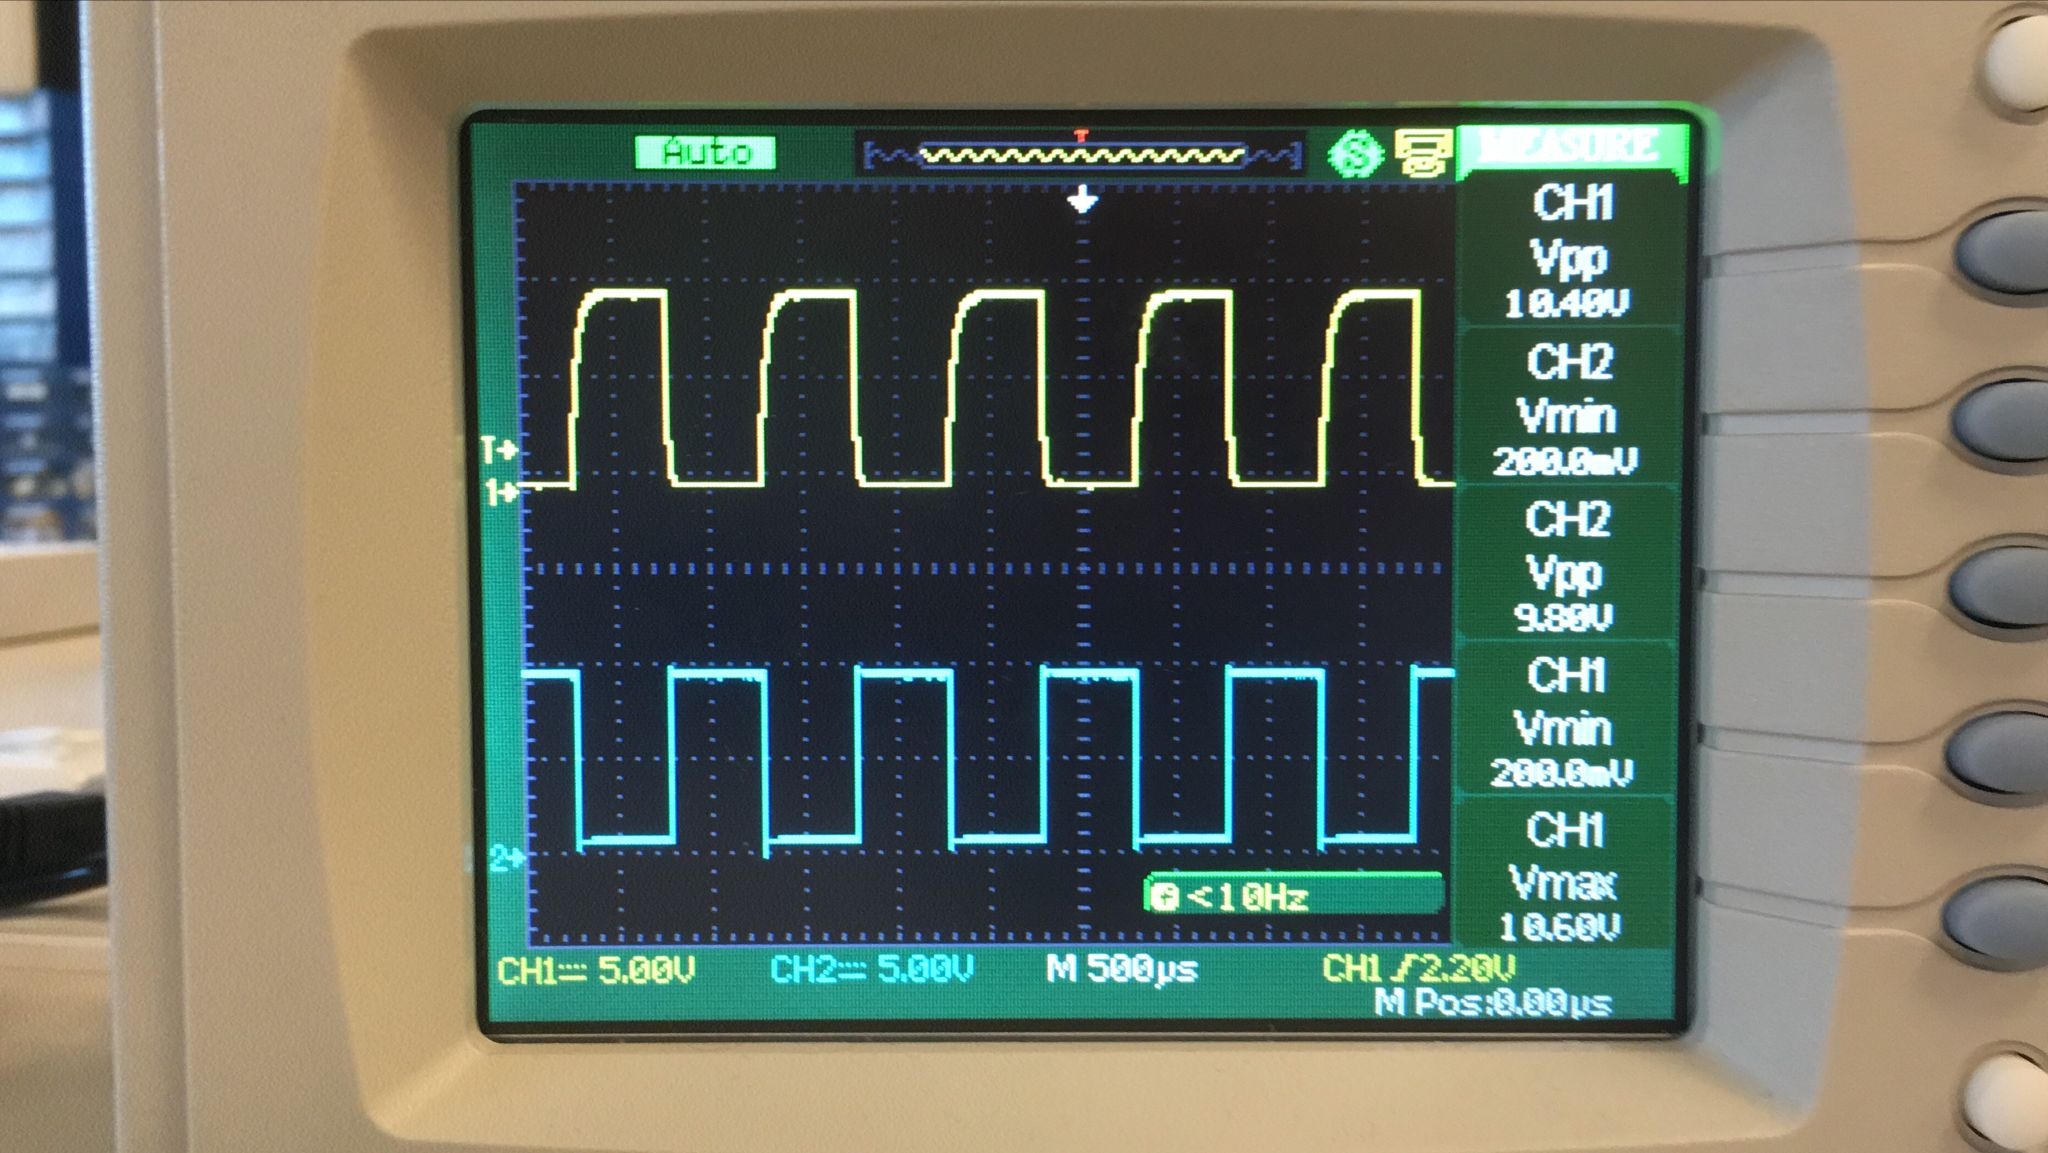
\includegraphics[width=0.7\linewidth]{images/task1_2.2uf.png}
    \caption{Inverter Waveform with $2.2\ \mu\text{F}$ Capacitive Load}
\end{figure}

The increase in capacitance directly increased the time constant ($\tau = RC$). Consequently, the slopes of the rising and falling edges became less steep. Although the output still reaches the full $10\text{V}$ and $0\text{V}$ rails, it takes a bit larger portion of the $0.5\text{ ms}$ half-period to do so.


\subsubsection*{Task 1.3: $220\ \mu\text{F}$ Capacitor Load}
Finally, a very large $220\ \mu\text{F}$ capacitor was placed at the output terminal. The recorded waveform is shown in Figure 3.

\begin{figure}[h]
        \centering
        % Replace with your image filename
        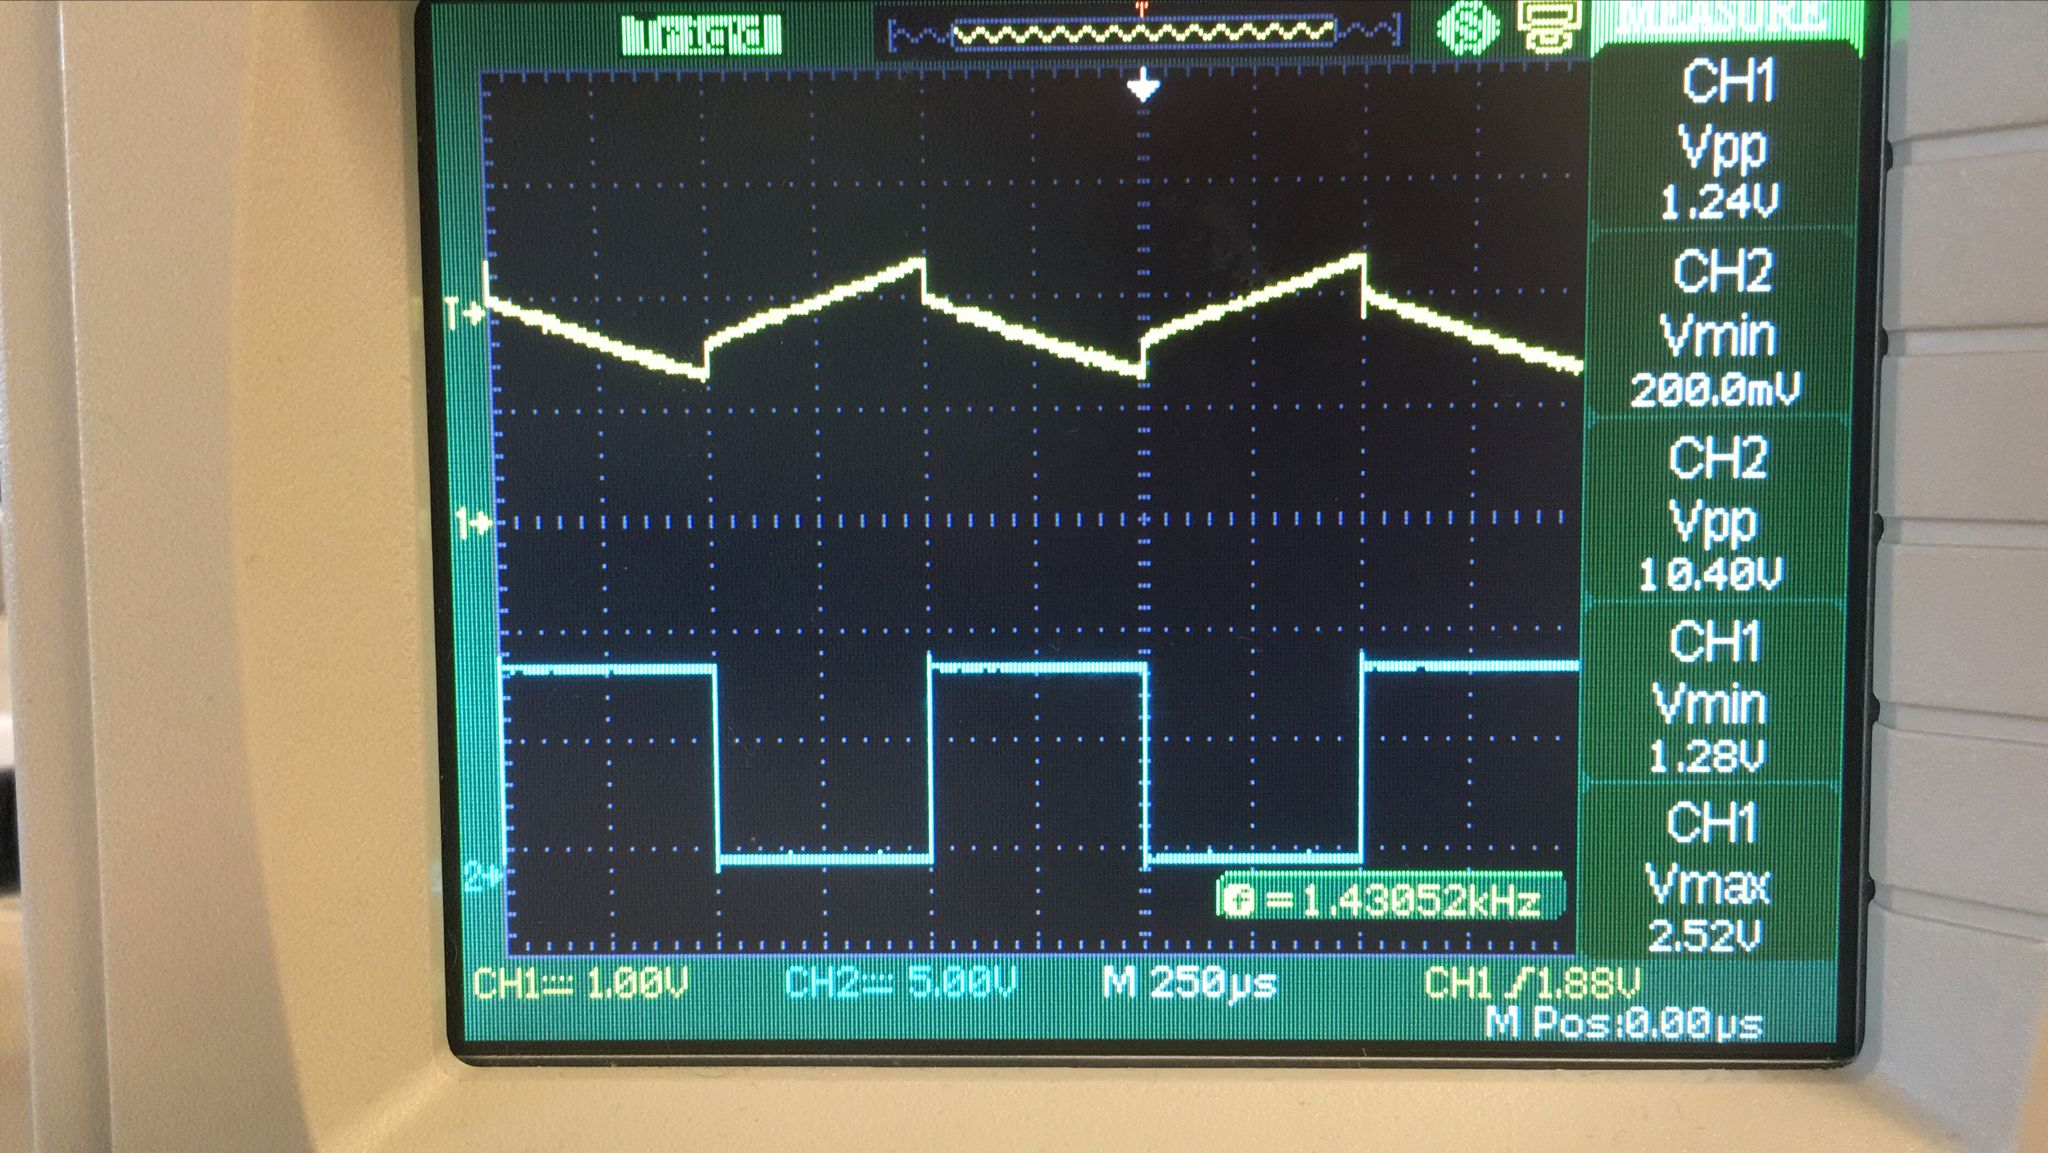
\includegraphics[width=0.7\linewidth]{images/task1_220uf.png}
    \caption{Inverter Waveform with $220\ \mu\text{F}$ Capacitive Load}
\end{figure}

With the $220\ \mu\text{F}$ capacitor, the output voltage failed to reach the full voltage swing. Because the time constant became excessively large relative to the $0.5\text{ ms}$ signal duration, the capacitor could only charge and discharge by a small fraction of the source voltage. The output waveform resembles a small triangular ripple centered around the switching threshold.

\subsubsection*{Analysis of Part 1}
The charging and discharging time of a capacitor in a CMOS circuit is governed by the relation $I = C \frac{dV}{dt}$. Because the discrete MOSFETs have a finite ON-resistance ($R_{on}$) and the power supply has a peak current limit, the output current is bounded. 
\begin{itemize}
    \item As the capacitance ($C$) increases, the rate of voltage change ($dV/dt$) decreases proportionately.
    \item For $1\ \mu\text{F}$ and $2.2\ \mu\text{F}$, the half-period of the $1\text{ kHz}$ signal ($0.5\text{ ms}$) is long enough for the output to fully settle.
    \item For $220\ \mu\text{F}$, the required time to fully charge is much longer than $0.5\text{ ms}$, resulting in heavily attenuated triangular-like output swings.
\end{itemize}

\newpage
\section*{Part 2: Ring Oscillator Using SN7404 NOT Gates}
In this section, a 3-stage ring oscillator was constructed using the SN7404 Hex Inverter IC. Because each gate has an inherent propagation delay, feeding the output of an odd number of stages back to the input creates an unstable state that oscillates at a frequency $f = 1/(2N\tau_p)$.

\subsection*{Task 2.1: 3-Stage Oscillator (Unbuffered)}
The ring was closed using three NOT gates. The oscilloscope probe was connected directly to the output of the third gate. 

\begin{figure}[h]
    \centering
    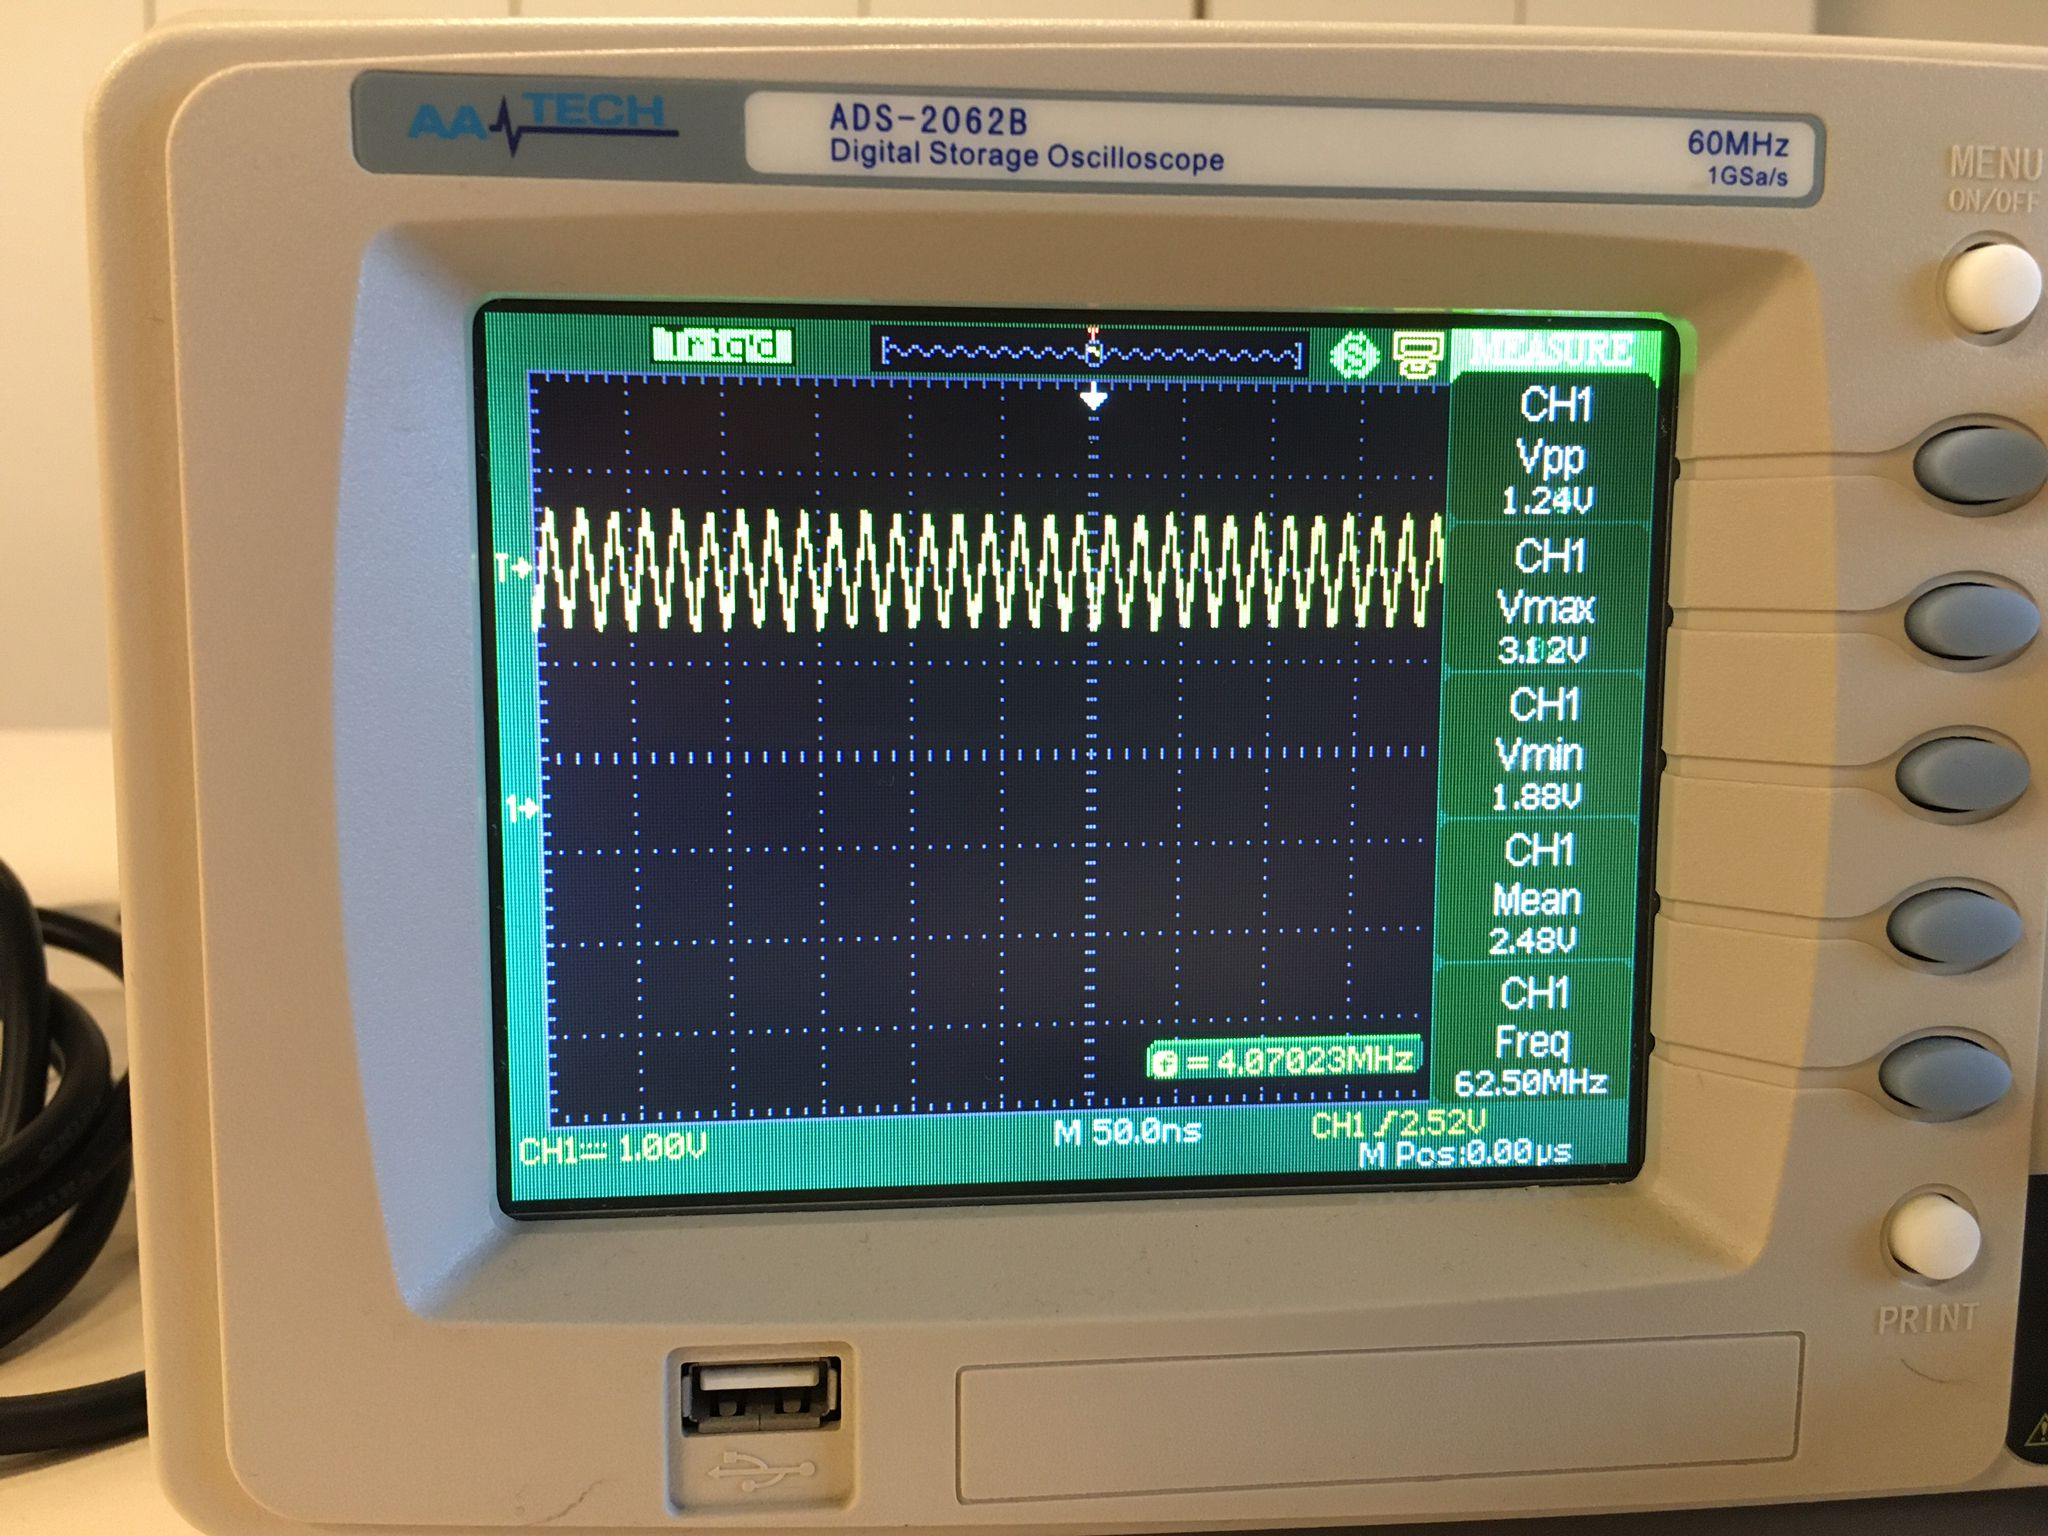
\includegraphics[width=0.7\linewidth]{images/task2_1.png}
    \caption{Oscilloscope waveform of the unbuffered ring oscillator.}
\end{figure}

The measurements recorded for the unbuffered output are as follows:
\begin{table}[h]
    \centering
    \begin{tabular}{lc}
        \toprule
        \textbf{Parameter} & \textbf{Measured Value} \\
        \midrule
        $V_{max}$ & 3.12 V \\
        $V_{min}$ & 1.88 V \\
        $V_{mean}$ & 2.48 V \\
        \bottomrule
    \end{tabular}
    \caption{Voltage parameters for Task 2.1}
\end{table}
\newpage
\subsection*{Task 2.2: 4th Stage Buffer Output}
A 4th NOT gate was added outside the feedback loop to act as a buffer. This gate isolates the oscillator from the probe's capacitance and resistance, which otherwise loads the circuit.

\begin{figure}[h]
    \centering
    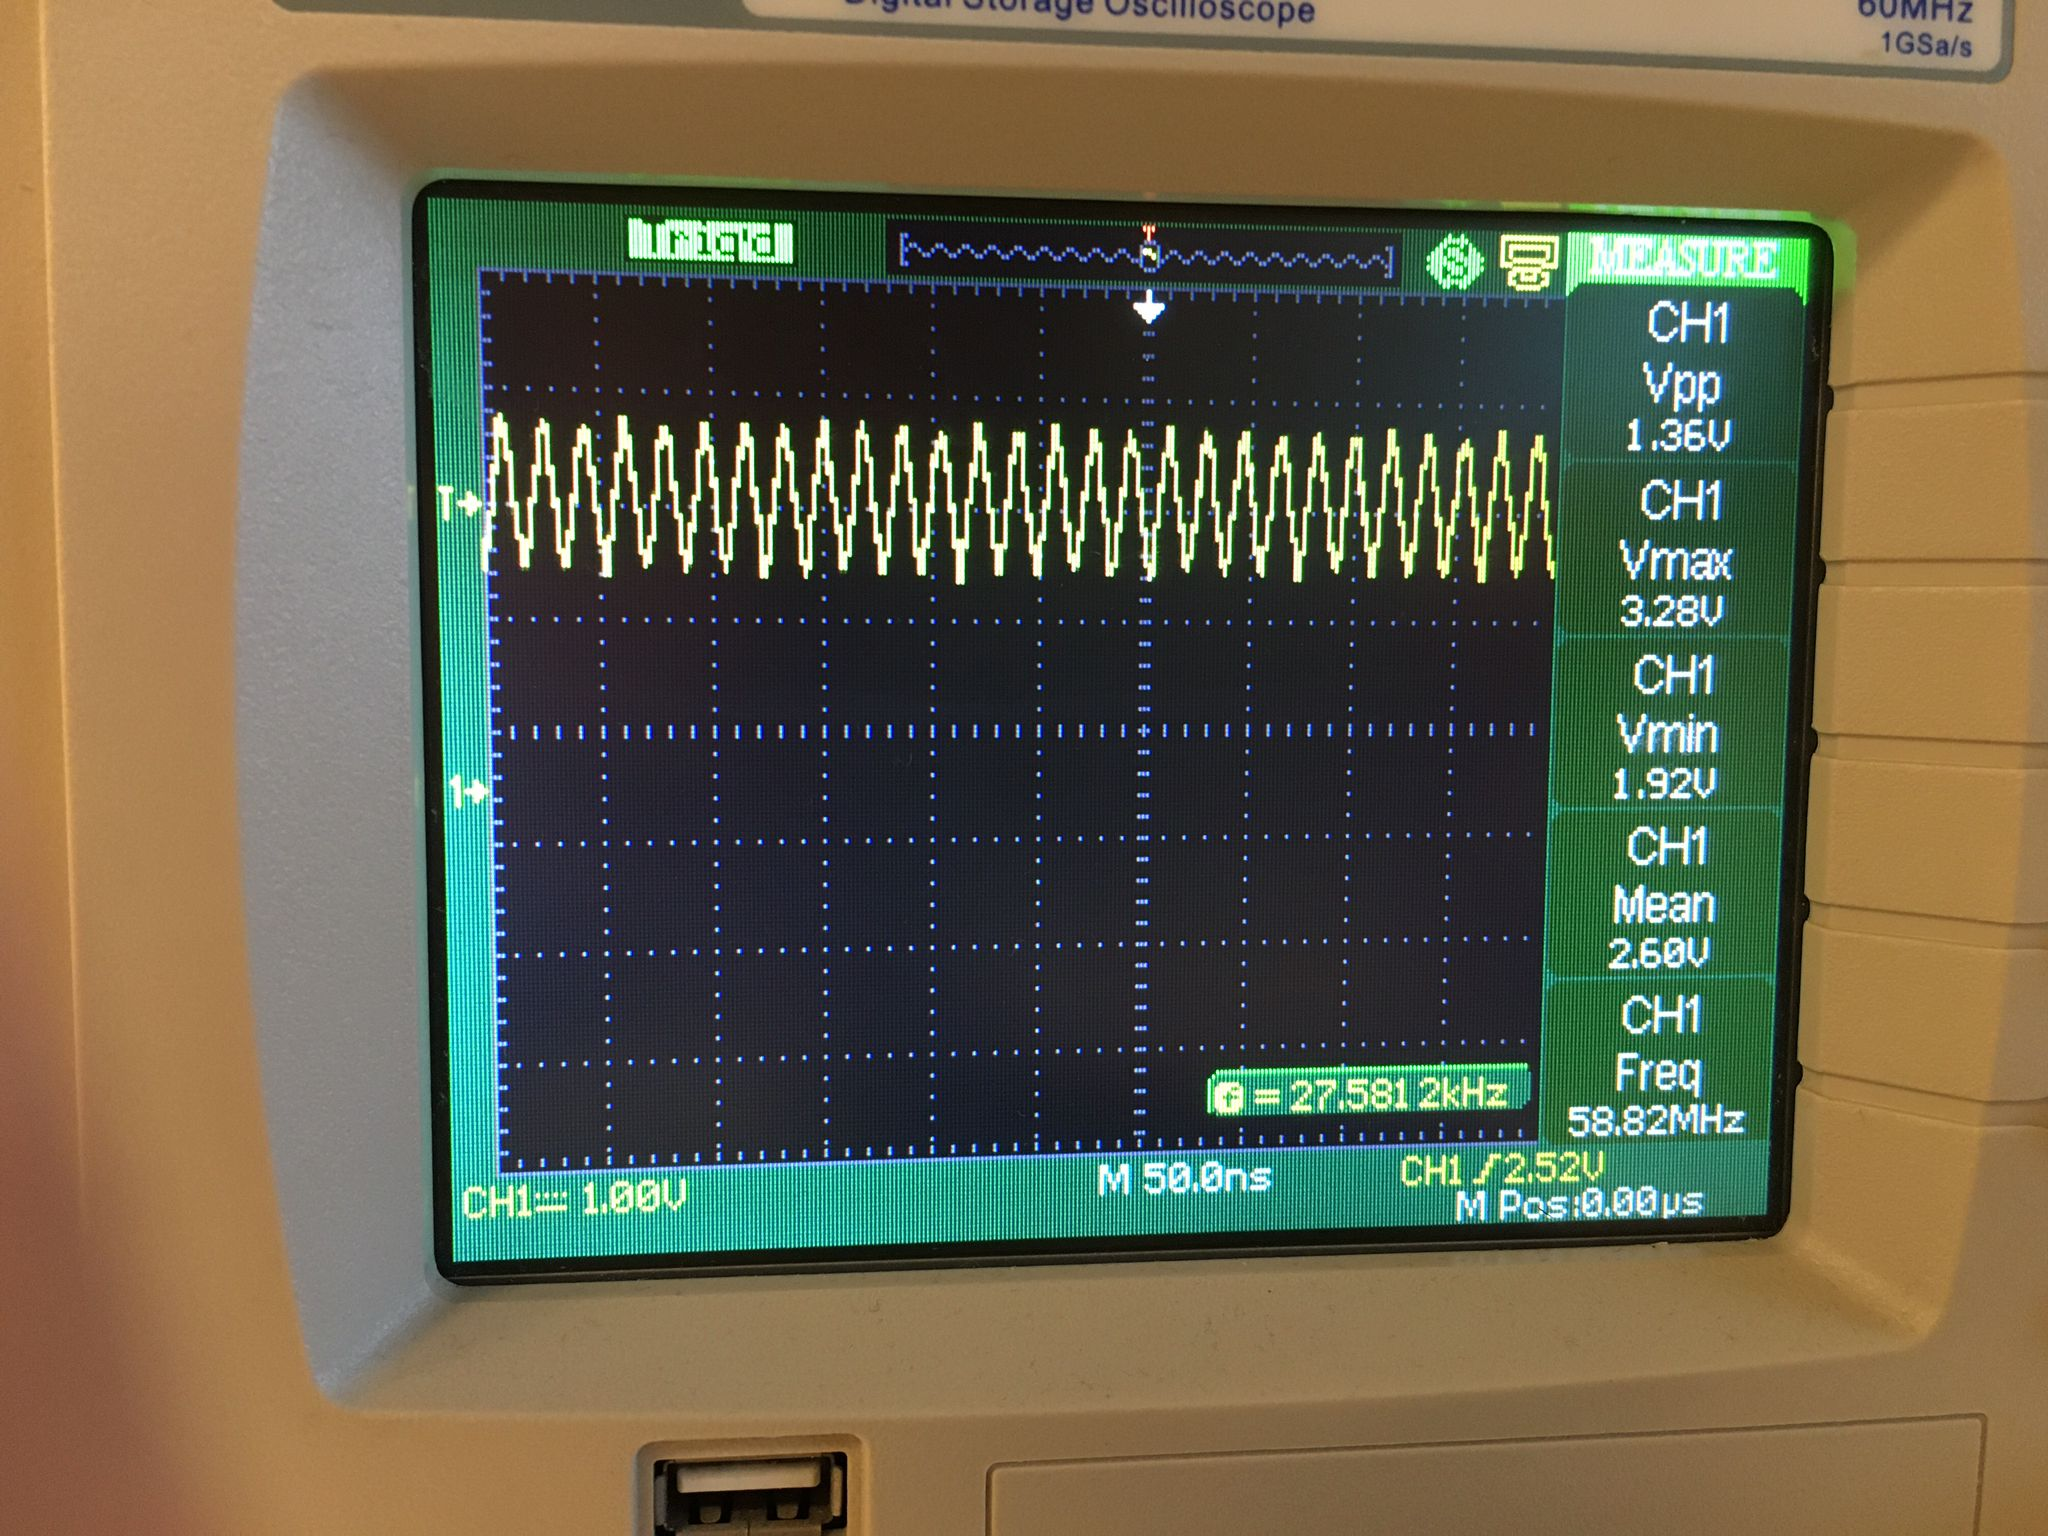
\includegraphics[width=0.7\linewidth]{images/task2_2.png}
    \caption{Oscilloscope waveform of the buffered ring oscillator output.}
\end{figure}

\begin{table}[h]
    \centering
    \begin{tabular}{lc}
        \toprule
        \textbf{Parameter} & \textbf{Measured Value} \\
        \midrule
        $V_{max}$ & 3.28 V \\
        $V_{min}$ & 1.92 V \\
        $V_{mean}$ & 2.60 V \\
        \bottomrule
    \end{tabular}
    \caption{Voltage parameters for Task 2.2}
\end{table}

\subsection*{Analysis and Comparison}
Comparing Task 2.1 and Task 2.2 reveals the impact of loading and buffering on high-frequency CMOS signals:

\begin{itemize}
    \item \textbf{Improved Voltage Swing:} The unbuffered peak-to-peak voltage ($V_{pp}$) was $1.24\text{V}$ ($3.12\text{V} - 1.88\text{V}$). Adding the buffer increased the swing to $1.36\text{V}$ ($3.28\text{V} - 1.92\text{V}$). This confirms that the buffer restores logic levels and provides a stronger drive capability.
    
    \item \textbf{Isolation from Loading:} The increase in $V_{max}$ from $3.12\text{V}$ to $3.28\text{V}$ indicates that the oscilloscope probe was loading the sensitive feedback loop. The buffer stage effectively isolates the oscillator from the probe's parasitic capacitance, allowing the ring to oscillate more freely.
    
    \item \textbf{Signal Symmetry:} In both cases, $V_{mean}$ remained near $2.5\text{V}$ ($V_{CC}/2$). This confirms that the waveform is oscillating symmetrically around the switching threshold of the SN7404 inverters.
\end{itemize}

\section*{Conclusion}

In this experiment, key characteristics of CMOS digital circuits were analyzed practically:
\begin{itemize}
    \item \textbf{Capacitive Loading on Inverters:} We verified that increasing the load capacitance severely degrades the switching speed of a CMOS inverter. At extreme loads ($220\ \mu\text{F}$), the output loses its ability to achieve full rail-to-rail logic levels.
    \item \textbf{Ring Oscillator Dynamics:} We demonstrated that an odd number of inverters in a ring creates an unstable state that leads to sustained high-frequency oscillations. Furthermore, the experiment emphasized the importance of output buffering when working with physically small, low-drive integrated circuit gates.
\end{itemize}
Overall, the experiment provided a clear understanding of dynamic power constraints and delay properties inherent to CMOS digital systems.
\end{document}